\chapter{Supernova Neutrino Bursts and Low-energy Neutrinos}
\label{ch:physics-snblowe}

\section{Overview}
\label{sec:physics-snblowe-overview}

The DUNE experiment will be sensitive to neutrinos in the few to few
tens of MeV range, which create short tracks potentially accompanied
gamma ray and other secondary particle signatures.  This regime is of
particular interest for detection of the burst of neutrinos from a
core-collapse supernova (the primary focus of this section), and
neutrinos from other astrophysical sources are also potentially detectable.
The low-energy event regime has particular reconstruction, background and triggering challenges.

\subsection{Expected  Signal}

A core-collapse supernova\footnote{``Supernova'' always
  refers to a ``core-collapse supernova'' in this chapter unless
  stated otherwise.} occurs when a massive star reaches the end of its
life, and stellar burning can no longer support the star's weight.
This catastrophic collapse results in a compact remnant such as a
neutron star, or possibly a black hole, depending on the mass of the
progenitor.  The infall is followed by a ``bounce'' when sufficiently
high core density is reached, and in some unknown (but non-zero)
fraction of cases, the shock wave formed after the bounce results in a
bright explosion~\cite{Janka:2012wk}.  The explosion energy represents
only a small fraction of the enormous total gravitational binding
energy of the resulting compact remnant, however --- thanks to the
neutrinos' weak coupling, which allows them to escape --- within a few
tens of seconds almost all of the energy is emitted in the form of
neutrinos in the tens-of-MeV range.  In spite of their weak coupling,
the neutrinos are copious enough to (very likely) play a significant
role in the explosion.

Neutrinos from the celebrated SN1987A core
collapse~\cite{Bionta:1987qt,Hirata:1987hu} in the Large Magellanic
Cloud outside the Milky Way were observed; however, the
statistics %of this observation
were sparse %enough that
and a great many questions remain.  A high-statistics observation of a
nearby supernova neutrino burst would be possible with the current
generation of detectors. Such an observation would shed light
on %very many questions about
the nature of the astrophysical event, as well as on the nature of
neutrinos themselves.  Sensitivity to the different flavor components
of the flux is highly desirable.

The core-collapse neutrino signal starts with a short, sharp
\emph{neutronization} (or \emph{break-out}) burst primarily composed of
$\nu_e$ (originating from $p+e^- \rightarrow n + \nu_e$, as protons
and electrons get squeezed together), and is followed by an
``accretion'' phase lasting some hundreds of milliseconds, as matter falls onto the collapsed core.  The later
``cooling'' phase over $\sim$10~seconds represents the main part of
the signal, over which the proto-neutron star sheds its gravitational
binding energy.  The neutrino flavor content and spectra change
throughout these phases, and the supernova's temperature evolution can
be followed with the neutrino signal.
% (see
%Figure~\ref{fig:temp_comparison}). 
Some fairly generic supernova
signal features are illustrated in Figure~\ref{fig:spectrum}, based on~\cite{Fischer:2009af} and reproduced from~\cite{Wurm:2011zn}.
% Last three cases can be quite complicated, especially last
%
\begin{figure}[!htb]
\centering
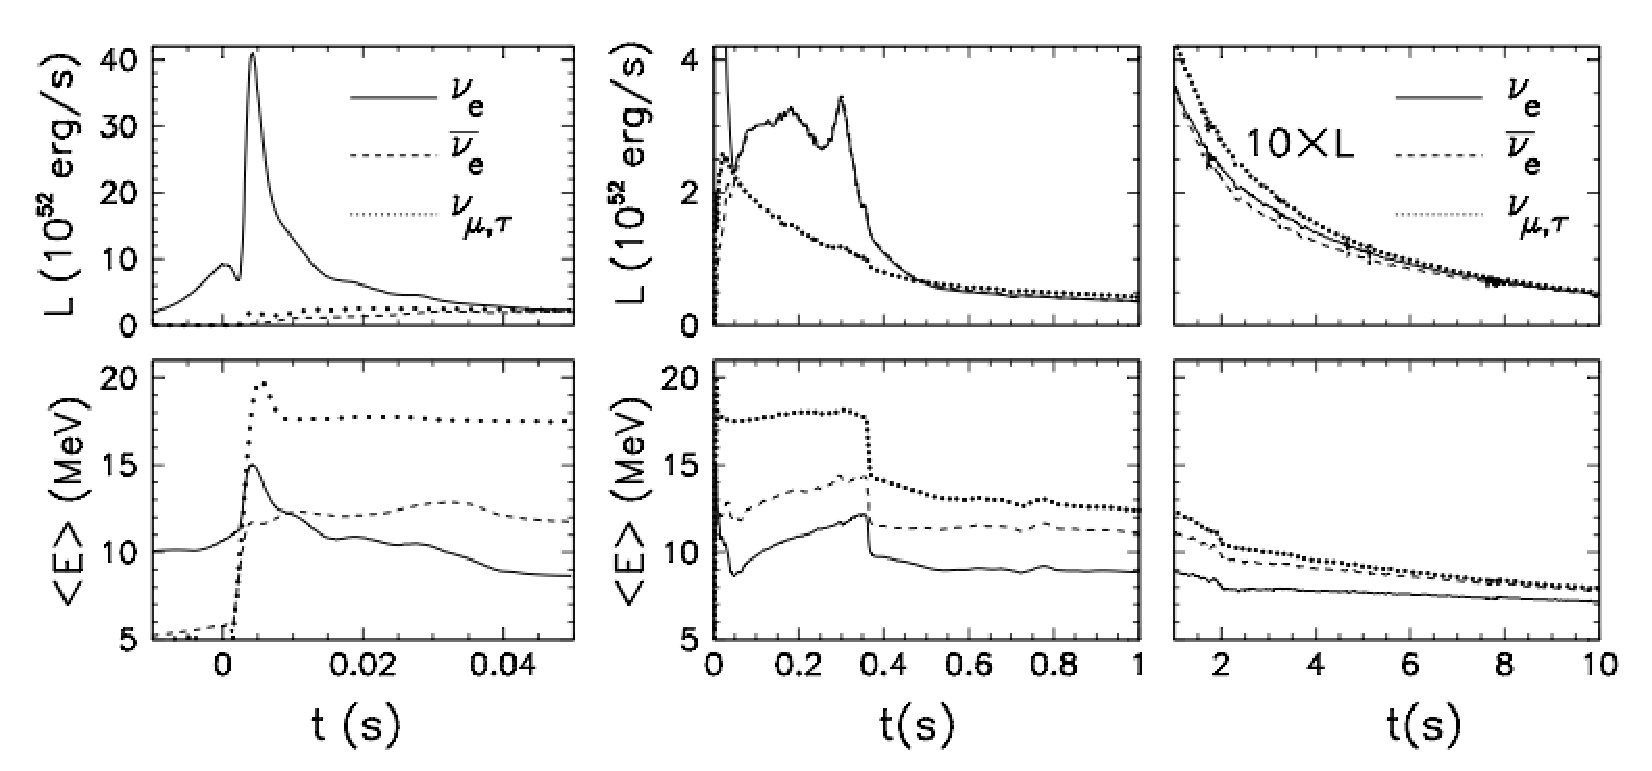
\includegraphics[width=0.9\textwidth]{basel_flux.pdf}
\caption[Expected core-collapse neutrino signal]{Expected
  core-collapse neutrino signal from the ``Basel''
  model~\cite{Fischer:2009af}, for a
  10.8 $M_{\cdot}$ progenitor.  The left plots show the very early
  signal, including ``neutronization burst;'' the middle plots show
  the ``accretion phase'', and the right plots show the cooling
  phase. Across the top, luminosities as a function of time are shown. 
  Across the bottom, the plots show average energy as a function of time for the
  $\nu_e$, $\overline{\nu}_e$ and $\nu_{\mu,\tau}$ flavor components of the
  flux (fluxes for $\nu_\mu$, $\overline{\nu}_\mu$, $\nu_\tau$,
  and $\overline{\nu}_\tau$ should be identical).  Figure courtesy of~\cite{Wurm:2011zn}.}
\label{fig:spectrum}
\end{figure}

The supernova neutrino spectrum at a given moment in time is expected
to be well described by a
parameterization~\cite{Minakata:2008nc,Tamborra:2012ac} given by:
\begin{equation}
        \label{eq:pinched}
        \phi(E_{\nu}) = \mathcal{N} 
        \left(\frac{E_{\nu}}{\langle E_{\nu} \rangle}\right)^{\alpha} \exp\left[-\left(\alpha + 1\right)\frac{E_{\nu}}{\langle E_{\nu} \rangle}\right] \ ,
\end{equation}
where $E_{\nu}$ is the neutrino energy, $\langle E_\nu \rangle$ is the
mean neutrino energy, $\alpha$ is a ``pinching parameter'', and
$\mathcal{N}$ is a normalization constant.
%
Large $\alpha$ corresponds to a more ``pinched'' spectrum (suppressed
high-energy tail). This parameterization is referred to as a
``pinched-thermal'' form. The different $\nu_e$, $\overline{\nu}_e$ and
$\nu_x, \, x = \mu, \tau$ flavors are expected to have different
average energy and $\alpha$ parameters and to evolve differently in
time. 


\subsection{Detection Channels and Interaction Rates}

Luquid argon should have a particular sensitivity to the $\nu_e$
component of a supernova neutrino burst, via charged-current
absorption of $\nu_e$ on $^{40}$Ar.  Cross sections for the most
relevant interactions are shown in Fig.~\ref{fig:xscns}.
% I have some improved figures somewhere...

\begin{figure}[!htb]
\centering
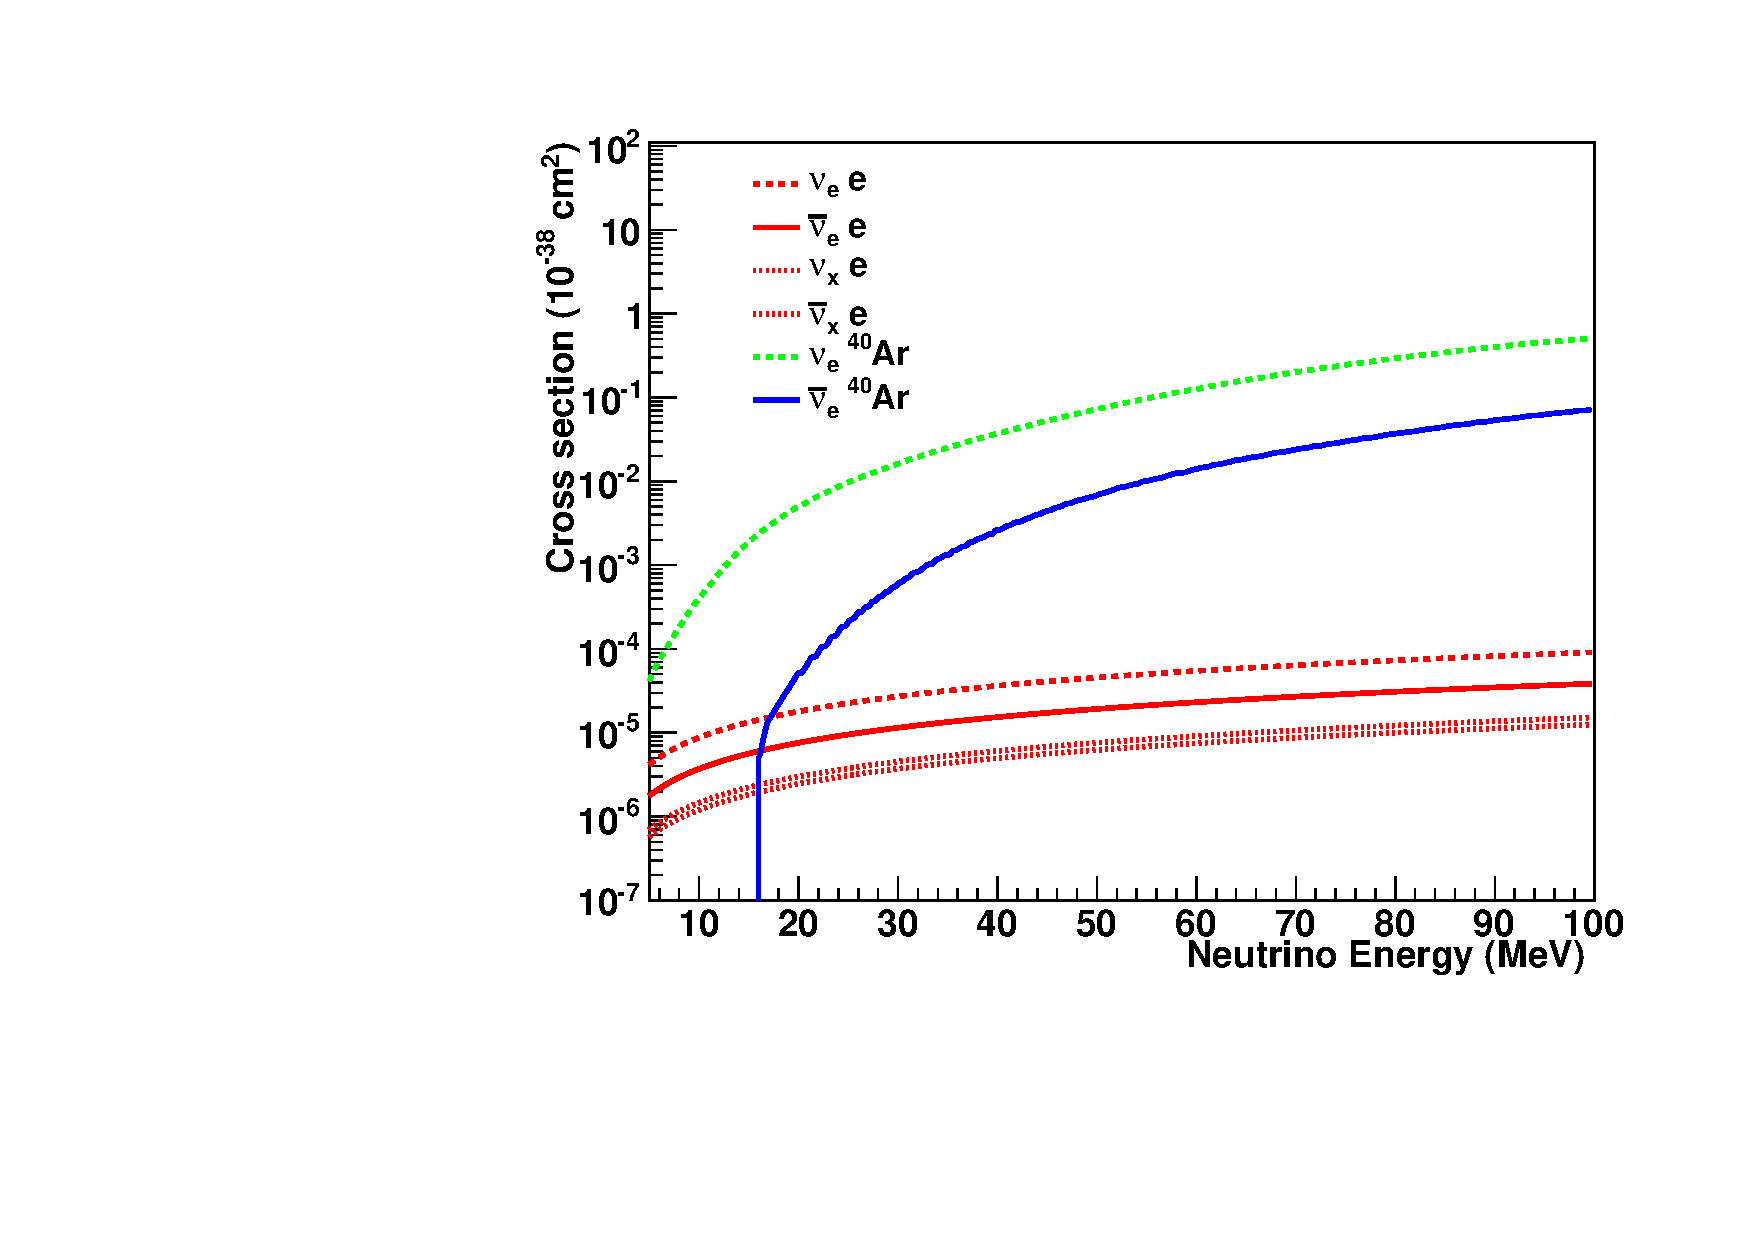
\includegraphics[width=0.6\textwidth]{argon_xscn.pdf}
\caption[]{Cross sections for supernova-relevant interactions in argon.}
\label{fig:xscns}
\end{figure}
%
The predicted event rate from a supernova burst may be calculated by
folding expected neutrino differential energy spectra in with cross
sections for the relevant channels, and with detector response.
%


Table~\ref{tab:argon_events} shows rates calculated  for the dominant interactions in argon for
the ``Livermore'' model~\cite{Totani:1997vj}, and the ``GKVM''
model~\cite{Gava:2009pj}.  Figure~\ref{fig:eventrates} shows the
expected observed differential event spectra for these fluxes.  Clearly, the $\nu_e$
flavor dominates.
%
\begin{table}[!htb]
  \caption[Event rates for different models in \SI{34}{\kt} of LAr for
    a core-collapse at 10~kpc]{Event rates for different
    supernova models in \SI{34}{\kt} of liquid argon for a core collapse at 10~kpc, for $\nu_e$ and $\bar{\nu}_e$ charged-current channels and elastic scattering (ES) on electrons.
    Event rates will simply scale by active detector mass and inverse square of supernova distance.}
\label{tab:argon_events}\centering
\begin{tabular}{$L^c^c}%$
\toprule
\rowtitlestyle
Channel & Events & Events \\
\rowtitlestyle
& ``Livermore'' model & ``GKVM'' model  \\ 
\toprowrule

$\nu_e + ^{40}{\rm Ar} \rightarrow e^- + ^{40}{\rm K^*}$ & 2308  & 2848 \\ \colhline

$\overline{\nu}_e + ^{40}{\rm Ar} \rightarrow e^+ + ^{40}{\rm Cl^*}$ & 194 & 134\\ \colhline

$\nu_x + e^- \rightarrow \nu_x + e^-$                           & 296 &  178\\

%$\nu_x + ^{40}{\rm Ar} \rightarrow \nu_x+ ^{40}{\rm Ar}^*$ & & \\ \hline
\toprule
\rowtitlestyle
Total &  2794& 3160 \\ 
\bottomrule
\end{tabular}
\end{table}
%
\begin{figure}[!htb]
\centering
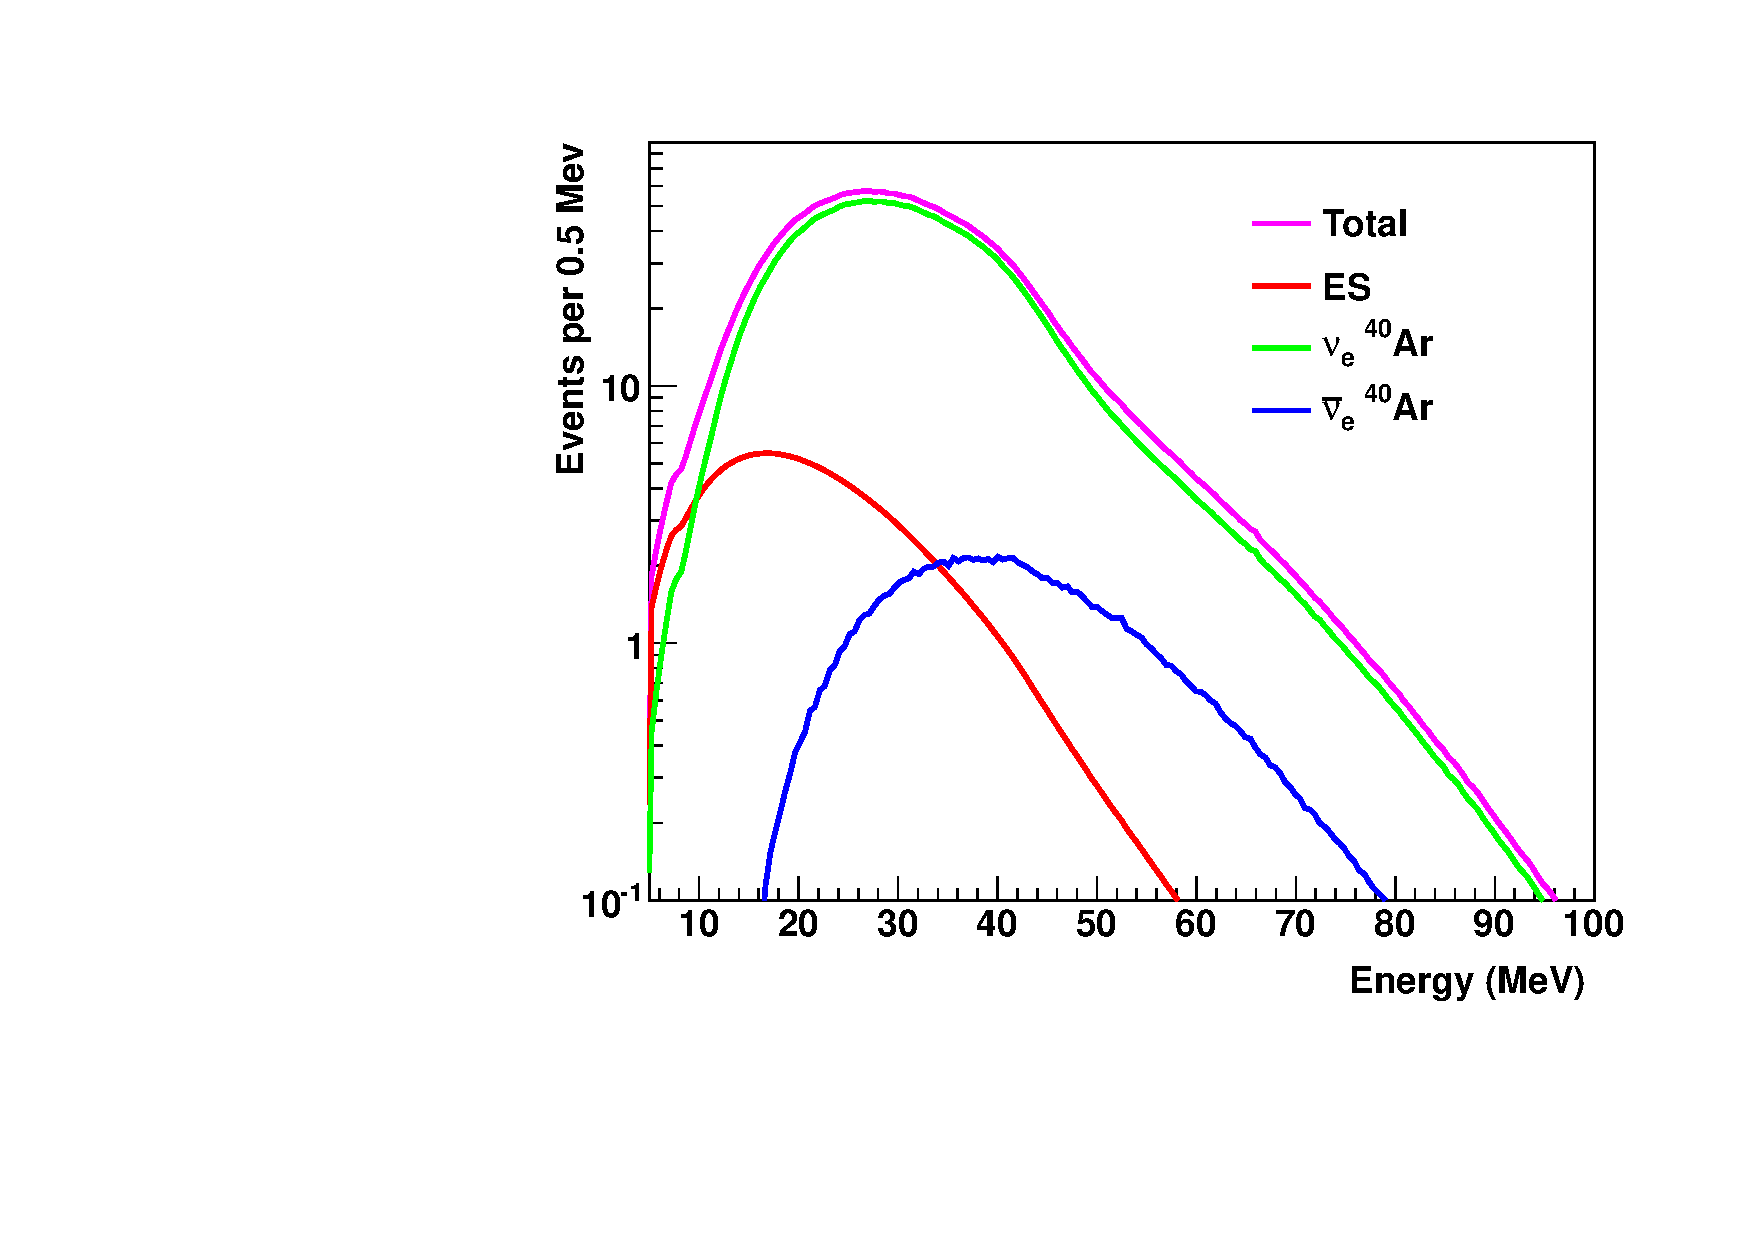
\includegraphics[width=2.0in]{interaction_rates_gvkm_ar34kt.pdf}
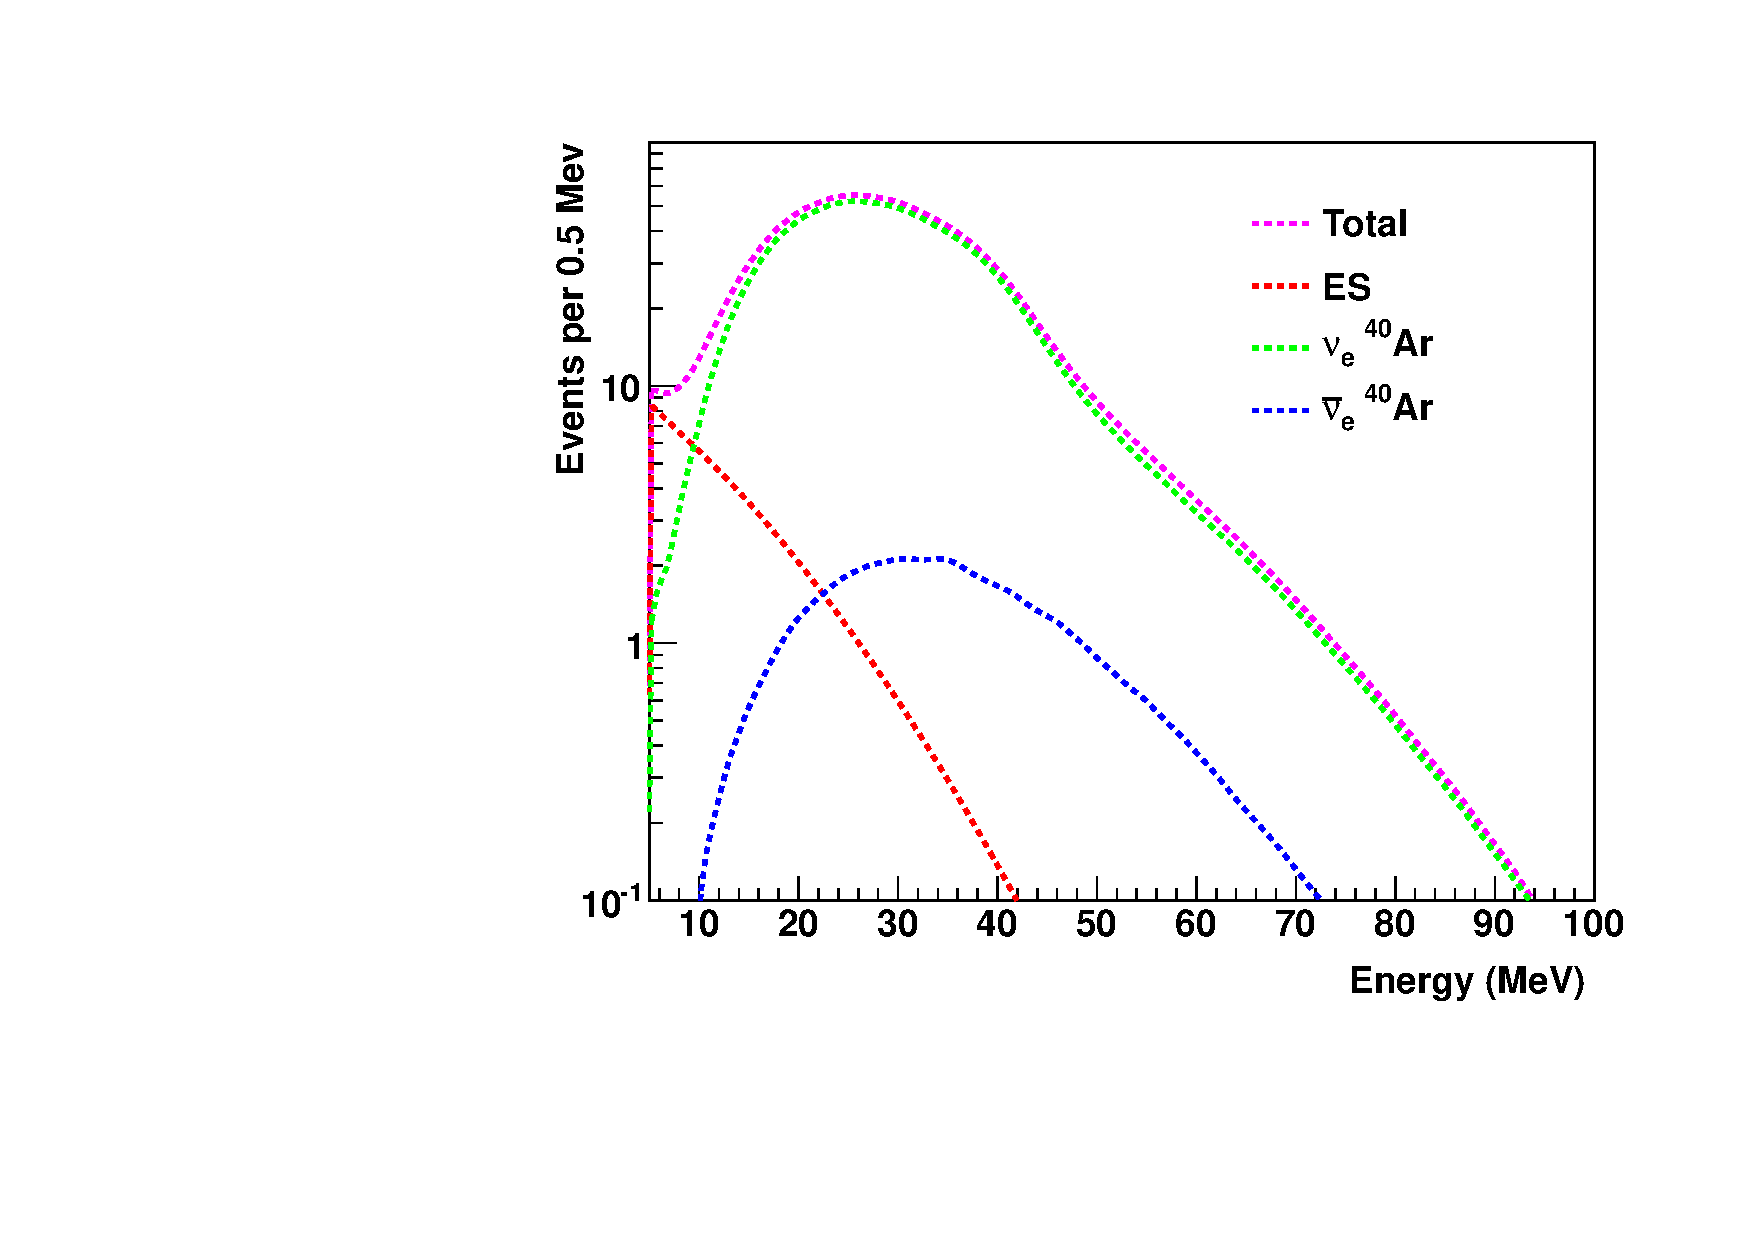
\includegraphics[width=2.0in]{smeared_rates_gvkm_ar34kt.pdf}
\vspace{-5pt}
\caption[SN $\nu$ event rates in \SI{34}{kt} of LAr for a core
  collapse at 10~kpc, GKVM]{Supernova neutrino event rates in 34~kt of argon for a core
  collapse at 10~kpc, for the GKVM model~\cite{Gava:2009pj} (events
  per 0.5~MeV), showing three relevant interaction channels. Left:
  interaction rates as function of true neutrino energy.  Right:
  ``smeared'' rates as a function of detected energy, assuming
  resolution from~\cite{Amoruso:2003sw}.}
  \label{fig:eventrates}
\end{figure}

Figure~\ref{fig:garching} gives another example of an expected burst
signal, for which a calculation with detailed time dependence of the
spectra is available~\cite{Huedepohl:2009wh} out to 9~seconds
post-bounce.  This model has relatively low luminosity but a robust
neutronization burst.  Note that the relative fraction of
neutronization-burst events is quite high.
%
\begin{figure}[!htb]
\centering
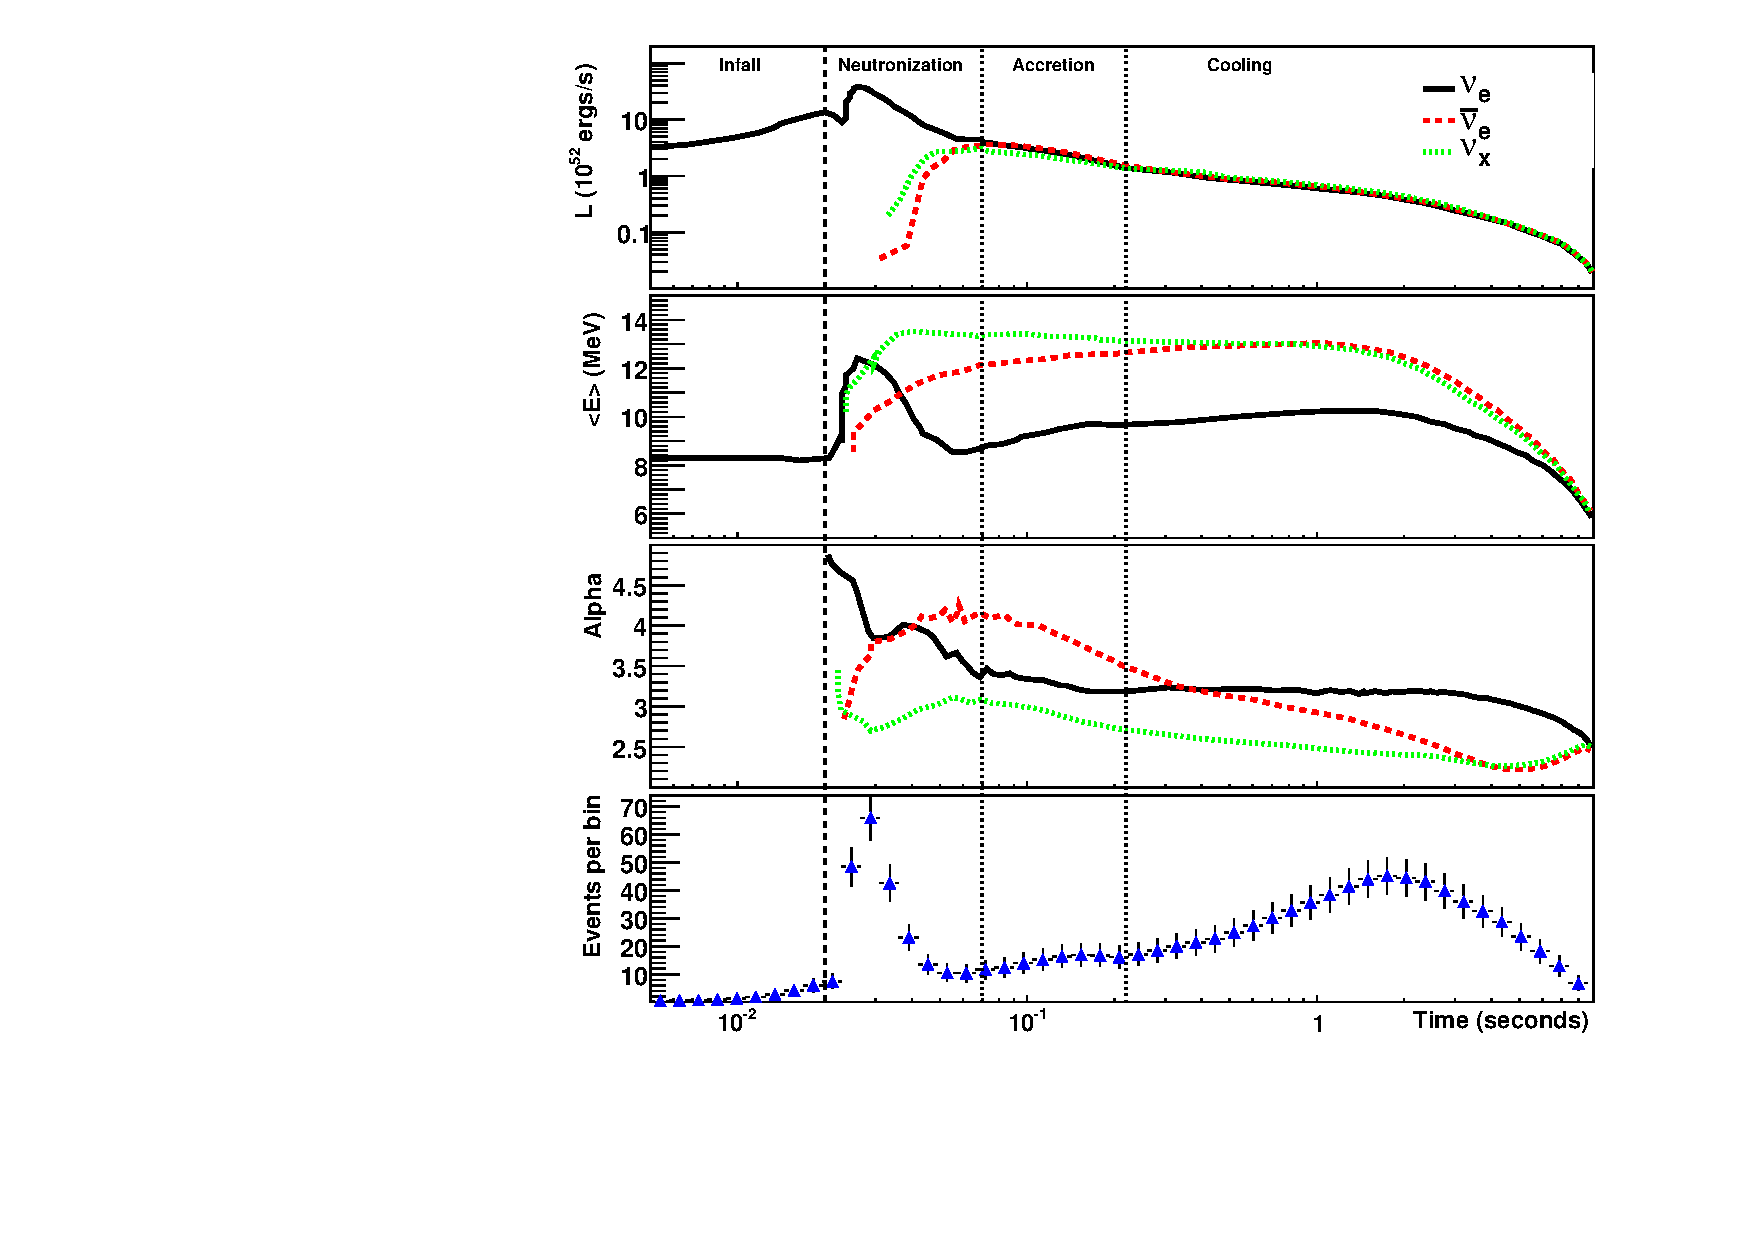
\includegraphics[width=0.9\textwidth]{garching.pdf}
\caption[Garching flux signal with neutronization burst]{ Expected
  time-dependent signal for a specific flux model for an
  electron-capture supernova~\cite{Huedepohl:2009wh} at 10~kpc.  The
  top plot shows the luminosity as a function of time, the second plot
  shows average neutrino energy, and the third plot shows the $\alpha$
  (pinching) parameter.  The fourth (bottom) plot shows the total number of
  events (mostly $\nu_e$) expected in 34 kt of liquid argon, calculated using
  SNoWGLoBES.  Note the logarithmic binning in time; the plot shows
  the number of events expected in the given bin and the error bars
  are statistical. The vertical dashed line at 0.02 seconds indicates
  the time of core bounce, and the vertical lines indicate different
  eras in the supernova evolution.  The leftmost time interval
  indicates the infall period.  The next interval, from core bounce to
  50~ms, is the neutronization burst era, in which the flux is
  composed primarily of $\nu_e$.  The next period, from 50 to 200~ms,
  is the accretion period. The final era, from 0.2 to 9~seconds, is
  the proto-neutron-star cooling period.  }
\label{fig:garching}
\end{figure}


\section{Neutrino Physics and Other Particle Physics}
\label{sec:physics-snblowe-neutrino-physics}


Neutrino oscillations modulate the flavor-energy-time evolution of the spectrum, including 
``collective'' effects due to neutrino-neutrino interactions.  A
voluminous literature exists exploring these collective phenomena,
e.g.,~\cite{Duan:2005cp,Fogli:2007bk,Raffelt:2007cb,Raffelt:2007xt,EstebanPretel:2008ni,Duan:2009cd,Dasgupta:2009mg,Duan:2010bg,Duan:2010bf}.

\textit{Update, more here}

Certain phenomena are even postulated to indicate
beyond-the-standard-model physics~\cite{Raffelt:1999tx} such as
axions, extra dimensions and an anomalous neutrino magnetic moment;
non-observation of these effects, conversely, would enable constraints
on these phenomena.


\textit{Add: absolute mass}

\textit{Add: LIV}

\section{Astrophysics}
\label{sec:physics-snblowe-astrophysics}



A number of astrophysical phenomena associated with supernovae are expected to be observable
in the supernova neutrino signal, providing a remarkable window into the event, for example: 
\begin{itemize}
\item The initial burst, primarily composed of $\nu_e$ and called the
  ``neutronization'' or ``breakout''
  burst, %should be observable, although it
  represents only a small component of the total signal.  However,
  oscillation effects can manifest themselves in an observable manner
  in this burst, and flavor transformations can be modified by the
  ``halo'' of neutrinos generated in the supernova envelope by
  scattering~\cite{Cherry:2013mv}.
\item The formation of a black hole would cause a sharp signal cutoff
  (e.g.,~\cite{Beacom:2000qy,Fischer:2008rh}).
\item Shock wave effects (e.g.,~\cite{Schirato:2002tg}) would cause a
  time-dependent change in flavor and spectral composition as the
  shock wave propagates.
\item The standing accretion shock instability
  (SASI)~\cite{Hanke:2011jf,Hanke:2013ena}, a ``sloshing'' mode
  predicted by three-dimensional neutrino-hydrodynamics simulations of
  supernova cores, would give an oscillatory flavor-dependent
  modulation of the flux.
\item Turbulence effects~\cite{Friedland:2006ta,Lund:2013uta} would
  also cause flavor-dependent spectral modification as a function of
  time.
\end{itemize}

The supernova neutrino burst is prompt with respect to the
electromagnetic signal and therefore can be exploited to provide an
early warning to astronomers~\cite{Antonioli:2004zb,Scholberg:2008fa}.
Additionally, a liquid argon signal~\cite{Bueno:2003ei} is expected to
provide some pointing information, primarily from elastic scattering
on electrons.

Even non-observation of a burst, or non-observation of
a $\nu_e$ component of a burst in the presence of supernovae (or other
astrophysical events) observed in electromagnetic or gravitational
wave channels, would still provide valuable information about the
nature of the sources.  Further, a long-timescale, sensitive search
yielding no bursts will also provide limits on the rate of
core-collapse supernovae.


% r-process

\section{Detector Requirements}
\label{sec:physics-snblowe-detector-requirements}

This may need more than the 1 page allocated.

Energy Resolution

Time Resolution

Angular Resolution

Particle ID, tagging

Backgrounds

Triggering, DAQ, Data Rate


\section{Additional Astrophysical Neutrinos}
\label{sec:physics-snblowe-other}

\subsection{Other Transient Neutrino Sources}

GRB, accretion disks...

\subsection{Diffuse Background Neutrinos}

\subsection{Solar Neutrinos}

\subsection{Dark Matter-Induced Neutrinos}

Might be more appropriate for atmnu-pdk... but boosted dark matter,
some other possibilities
